\normaltrue \difficilefalse \tdifficilefalse
\correctionfalse

%\UPSTIidClasse{11} % 11 sup, 12 spé
%\newcommand{\UPSTIidClasse}{12}

\exer{Banc Balafre $\star$ \label{B2:10:65}}
\setcounter{numques}{0}
\UPSTIcompetence[2]{B2-10}
\index{Compétence B2-10}
\index{Système éclipse}
\index{Matrice d'inertie}
\index{Caractéristiques inertielles}
\ifcorrection
\else
\textbf{Pas de corrigé pour cet exercice.}
\fi




\ifprof
\else

Les galets \textbf{2} et \textbf{3} sont de masses identiques $m_2$ et de centres d’inertie respectifs $G_2$ et $G_3$. Le balancier \textbf{1} est de masse \textbf{$m_1$} et de centre d’inertie $O$ (la tige de $G_3H$ étant de masse négligeable). 
Les solides \textbf{1}, \textbf{2} et \textbf{3} sont supposés homogènes (masse volumique notée $\mu$).
\begin{figure}[H]
\centering
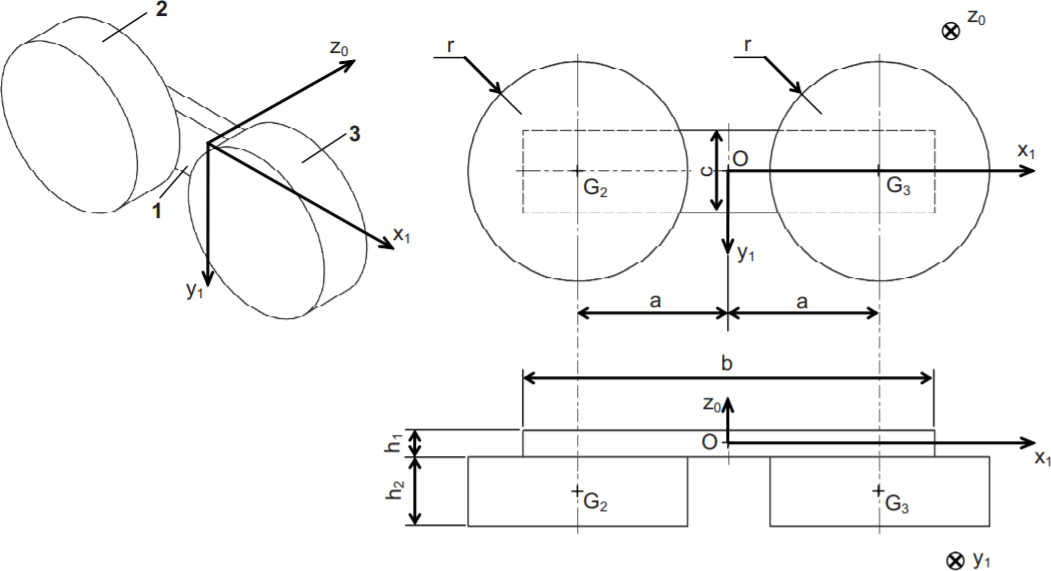
\includegraphics[width=\linewidth]{65_01}
\end{figure}
\fi

\question{Donner la forme de la matrice d’inertie du solide \textbf{1} au point \textbf{O} dans la base $\base{x_1}{y_1}{z_0}$.}
\ifprof
\else
\fi

\question{Exprimer littéralement le moment d’inertie $C_1$ du solide 1 par rapport à l’axe $\axe{O}{z_0}$, en fonction de la masse $m_1$ et de ses dimensions.}
\ifprof
\else
\fi

\question{Donner la forme de la matrice d’inertie du solide 2 au point $G_2$ dans la base
$\base{x_1}{y_1}{z_0}$.}
\ifprof
\else
\fi

\question{Exprimer littéralement le moment d’inertie $C'_2$ du solide 2 par rapport à l’axe $\axe{G_2}{z_0}$, en fonction de la masse $m_2$ et de ses dimensions.}
\ifprof
\else
\fi

\question{Exprimer littéralement le moment d’inertie $C_2$ du solide 2 par rapport à l’axe $\axe{G_2}{z_0}$, en fonction de la masse $m_2$ et de ses dimensions.}
\ifprof
\else
\fi






\ifprof
\else
\footnotesize
\begin{enumerate}
\item $\inertie{O}{1}=\matinertie{A_1}{B_1}{C_1}{0}{0}{0}{\base{x_1}{y_1}{z_0}}$.
\item $C_1 = \dfrac{m_1}{12}\left(b^2+c^2\right)$.
\item $\inertie{G_2}{1}=\matinertie{A_2}{A_2}{C_2}{0}{0}{0}{\base{x_1}{y_1}{z_0}}$.
\item $C'_2 =m_2\dfrac{r^2}{2}$.
\item $C_2 = m_2 \left(\dfrac{r^2}{2} +a^2 \right)$.
\end{enumerate}
\normalsize
\begin{flushright}
\footnotesize{Corrigé voir \ref{B2:10:65}.}
\end{flushright}%
\fi